\chapter{Geometry}
\section{G1 - Estimation of vanishing line of the horizontal plane}\label{infLine}
In projective geometry, a vanishing point is the image of a set of parallel lines in \verb|3D| space after projecting onto the \verb|2D| image plane. Although truly parallel lines in the scene never meet in Euclidean space, their perspective projection often appears to converge at a single point in the image.

Due to measurement noise and inaccuracies, different pairs of parallel lines will not intersect at a single precise point. Thus, a common strategy is to seek the point that minimizes the sum of squared distances between the measured image lines and a single convergent point, leading to a maximum likelihood estimate under Gaussian noise assumptions.

Although the initial request was to automatically extract straight lines, I opted to manually select all the required lines to achieve a more accurate and precise outcome.

\subsection[Vanishing Point of \textit{l} Lines]{Vanishing Point of $l_i$ Lines} \label{sec:vanPoint_l}
In the following section there will be presented two different approaches to estimate the vanishing point of $l_i$ lines. 

\subsubsection{Centroid-based Approach}
The centroid-based approach is a simple and computationally efficient method for estimating the vanishing point in an image. It involves computing the intersections of all pairs of image lines and taking the centroid (mean position) of these intersection points as the estimated vanishing point.

Despite its simplicity, the centroid method lacks robustness to noise and outliers, as all intersections are treated equally, including those from erroneously detected lines. As such, it is best suited for cases where line measurements are precise and free from significant outliers. For higher accuracy, more advanced methods, such as optimization-based techniques, are preferred.

\subsubsection{Levenberg-Marquardt Algorithm}
The Levenberg-Marquardt (LM) algorithm is a popular technique for solving non-linear least squares problems. It combines the best features of two optimization methods: the Gauss-Newton method and gradient descent.

\begin{itemize}
    \item \textbf{Gauss-Newton:} Efficient for problems that are well approximated by a quadratic near the solution, using the Jacobian and approximate second-order information.
    \item \textbf{Gradient Descent:} Robust for initial steps, but can be slow to converge.
\end{itemize}

LM smoothly transitions between these two approaches. When the solution is far from the optimum, LM behaves more like gradient descent, ensuring stability. As it gets closer to the optimum, it behaves more like Gauss-Newton, ensuring fast convergence. This makes LM a robust and efficient choice for a variety of parameter estimation problems, including camera calibration, structure-from-motion, and vanishing point estimation.

\subsubsection{Comparison and results}
In our scenario, the image data and detected lines exhibit relatively low levels of noise, as the parallel structures in the scene are well-defined and the line detections are accurate. As a result, the intersections of the lines cluster closely around the true vanishing point, minimizing the scatter typically caused by noise.

Given these favourable conditions, the centroid-based approach provides a computationally efficient and sufficiently accurate method for estimating the vanishing point. As demonstrated in the accompanying figure, the centroid of the pairwise line intersections aligns closely with the true vanishing point, delivering reliable results without requiring more complex optimization methods like the Levenberg-Marquardt algorithm.

While the LM algorithm offers improved robustness and precision in highly noisy or challenging datasets, in this case, its additional computational overhead is unnecessary. The simplicity and effectiveness of the centroid-based method make it the preferred choice for this specific scenario.

The vanishing points of $l$ lines we found:
$$
V_{l_{centroid}} = [3392.3, \, 666.4, \, 1]^T \qquad V_{l_{LM}} = [3416.8, \, 674.4, \, 1]^T
$$

The computed values are very similar; therefore, for the subsequent steps, we will use the $V_l$ value obtained through the centroid-based approach.

$$V_l = [3392.3, \, 666.4, \, 1]^T$$

\subsection[Vanishing Point of \textit{m} Lines]{Vanishing Point of $m_j$ Lines}
Similarly to the previous section and based on the result's comparison between LM approach and centroid-based one, I estimate the vanishing point of $m_j$ lines using the centroid based approach:

$$
V_m = [581.4, \, 883.8, \, 1]^T
$$

\subsection{Estimation of the line at infinity}
The task was to construct and visualize the \textbf{line at infinity} $l'_\infty$ in the image plane, given the coordinates of two vanishing points. 

The line passing through the two vanishing points is computed using \textbf{cross product}
$$l_\infty = V_l \times V_m$$
where $V_l$ and $V_m$ are represented in homogeneous coordinates.

The result vector $l'_\infty = [a, \, b, \, c]^T$ represents the line at infinity in homogeneous coordinates, where:
$$ax + by + c = 0$$

The obtained result is:
$$l'_\infty = [-0.0001, \, -0.0011, \, 1]^T $$
\begin{figure}[H]
    \centering
    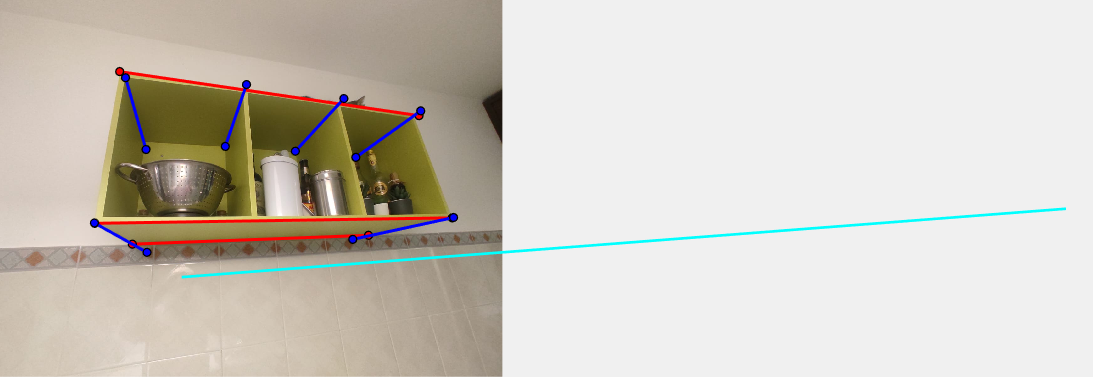
\includegraphics[width=0.95\linewidth]{img/G1/line_at_infinity.jpg}
    \caption{Line at Infinity}
    \label{fig:lineAtInfinity}
\end{figure}